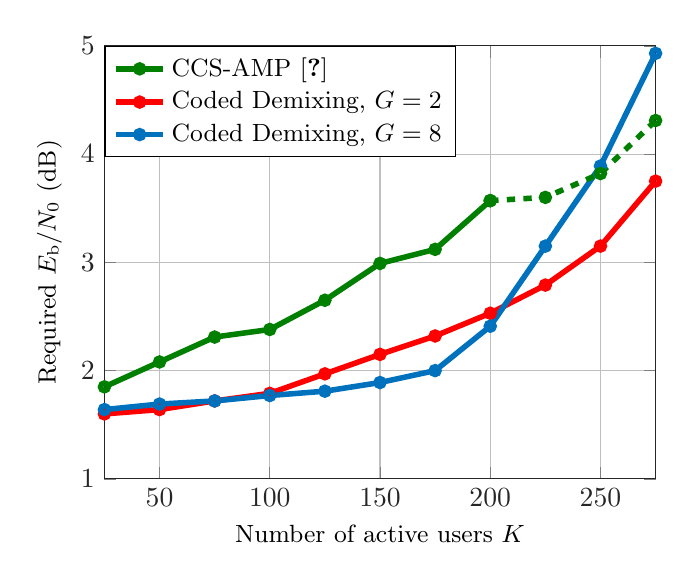
\begin{tikzpicture}

\definecolor{vamsired}{rgb}{0.63529,0.07843,0.18431} % red
\definecolor{vamsiblue}{rgb}{0.00000,0.44706,0.74118} % blue
\definecolor{vamsigreen}{rgb}{0.00000,0.49804,0.00000} % dark green
\definecolor{vamsiorange}{rgb}{0.87059,0.49020,0.00000} % orange
\definecolor{mycolor5}{rgb}{0.00000,0.44700,0.74100} %
\definecolor{mycolor6}{rgb}{0.74902,0.00000,0.74902} %

\begin{axis}[%
font=\small,
width=7cm,
height=5.5cm,
scale only axis,
every outer x axis line/.append style={white!15!black},
every x tick label/.append style={font=\color{white!15!black}},
xmin=25,
xmax=275,
xtick = {0,50,100,...,275},
xlabel={Number of active users $K$},
xmajorgrids,
every outer y axis line/.append style={white!15!black},
every y tick label/.append style={font=\color{white!15!black}},
ymin=1,
ymax=5,
ytick = {1,...,5},
ylabel={Required $E_{\mathrm{b}}/N_0$ (dB)},
ymajorgrids,
legend style={at={(0,1)},anchor=north west, draw=black,fill=white,legend cell align=left}
]

% \addplot [color=black,dotted,line width=1.5pt]
%   table[row sep=crcr]{
%  25	0.25\\
% 50	0.3\\
% 75	0.35\\
% 100	0.4\\
% 125	0.45\\
% 150	0.5\\
% 175	0.55\\
% 200	0.6\\
% 225	0.95\\
% 250	1.25\\
% 275	1.55\\
% % 300	1.8\\
% };
% \addlegendentry{Random Coding \cite{polyanskiy2017perspective}};

\addplot [color=vamsigreen,solid,line width=2.0pt,mark size=1.4pt,mark=o,mark options={solid}]
  table[row sep=crcr]{10 1.7 \\
25 1.85 \\
50 2.08 \\
75 2.31 \\
100 2.38 \\
125 2.65\\
150 2.99 \\
175 3.12 \\
200 3.57\\
% 225 3.6 \\
% 250 3.82 \\
% 275 4.31 \\
% 300 4.89 \\
};
\addlegendentry{CCS-AMP \cite{amalladinne2020unsourced}};

% JRE NOTE: this corresponds to the original curve. These results are outdated and sub-optimal
% \addplot [color=red, dashed,line width=2.0pt,mark size=1.4pt,mark=o,mark options={solid}]
% table[row sep=crcr]{
%   25 1.86 \\
%   50 1.92 \\
%   75 1.95 \\
%   100 2.05 \\
%   125 2.08 \\
%   150 2.24 \\
%   175 2.4 \\
%   200 2.6 \\
%   225 2.79 \\
%   250 3.15 \\
%   275 3.75 \\
% };
% \addlegendentry{Coded Demixing, $G = 2$};

% JRE Note: this corresponds to best-known results
\addplot [color=red, solid,line width=2.0pt,mark size=1.4pt,mark=o,mark options={solid}]
table[row sep=crcr]{
  25 1.60 \\
  50 1.64 \\
  75 1.72 \\
  100 1.79 \\
  125 1.97 \\
  150 2.15 \\
  175 2.32 \\
  200 2.53 \\
  225 2.79 \\
  250 3.15 \\
  275 3.75 \\
};
\addlegendentry{Coded Demixing, $G = 2$};

% JRE NOTE: this corresponds to the original curve. These results are outdated and sub-optimal
% \addplot [color=vamsiblue, dashed,line width=2.0pt,mark size=1.4pt,mark=o,mark options={solid}]
% table[row sep=crcr]{
%   25 1.71 \\
%   50 1.80 \\
%   75 1.83 \\
%   100 1.91 \\
%   125 1.98 \\
%   150 2.02 \\
%   175 2.13 \\
%   200 2.43 \\
%   225 3.15 \\
%   250 3.89 \\
%   275 4.93 \\
% };
% \addlegendentry{Coded Demixing, $G = 8$};

% JRE Note: this corresponds to best-known results
\addplot [color=vamsiblue, solid,line width=2.0pt,mark size=1.4pt,mark=o,mark options={solid}]
table[row sep=crcr]{
  25 1.64 \\
  50 1.691 \\
  75 1.72 \\
  100 1.77 \\
  125 1.81 \\
  150 1.89 \\
  175 2.00 \\
  200 2.41 \\
  225 3.15 \\
  250 3.89 \\
  275 4.93 \\
};
\addlegendentry{Coded Demixing, $G = 8$};

\addplot [color=vamsigreen,dashed,line width=2.0pt,mark size=1.4pt,mark=o,mark options={solid}]
  table[row sep=crcr]{
% 10 1.7 \\
% 25 1.85 \\
% 50 2.08 \\
% 75 2.31 \\
% 100 2.38 \\
% 125 2.65\\
% 150 2.99 \\
% 175 3.12 \\
200 3.57\\
225 3.6 \\
250 3.82 \\
275 4.31 \\
% 300 4.89 \\
};

\end{axis}
\end{tikzpicture}